\chapter{Experimental Procedure}
    This chapter explains how we prepared tools and devices for the purpose of experiments for our research work. We have used different third-party tools and frameworks, cloud-services like storages and runtime-machines. Finally, deployment of the trained model to android is also discussed here.
    
    \section{Preparing the Dataset}
        We have downloaded 380 web-scraped unique images with potholes from \href{https://kaggle.com}{\itshape{kaggle.com}} and more 285 images we have captured using an android-phone. This is shown in Table \ref{tab:img_sources}.
        
        \begin{table}[h]
            \centering
            \begin{tabular}{|c|c|c|} \hline
                Image Source &  Number of Images & Percentage \\\hline\hline
                Web-Scraping & 380 & 57.1\% \\\hline
                Camera-Capturing & 285 & 42.9\% \\\hline
            \end{tabular}
            \caption{Sources of Images Collected from}
            \label{tab:img_sources}
        \end{table}
        
        
        \vspace{1cm}
        In Figure \ref{fig:image_sources}, we have visualized the same thing using a 3D Pie-Chart.
        
        \begin{figure}
            \centering
            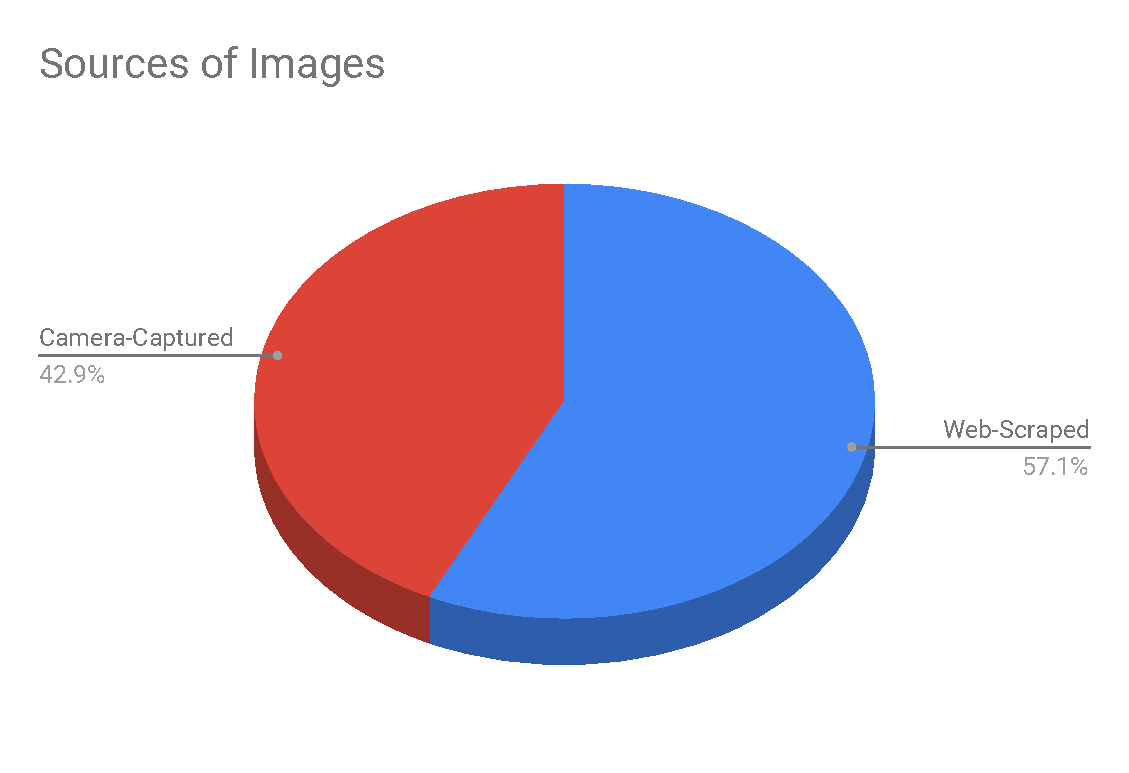
\includegraphics[width=\textwidth]{images/Sources of Images.pdf}
            \caption{Sources of Dataset Images}
            \label{fig:image_sources}
        \end{figure}
        
        \clearpage
        \subsection{Annotating the Regions of Interests}
            For detection of objects and things in images, in case of supervised learning, the regions of interests have to be annotated using bounding-boxes or image-segmentation with masking so that the training process can be accomplished.
            
            We have used \gls{labelimg} to select the regions of interests. This tool can generate \acrfull{xml} format file having the annotation details for each image.
        
            \begin{figure}[h]
                \centering
                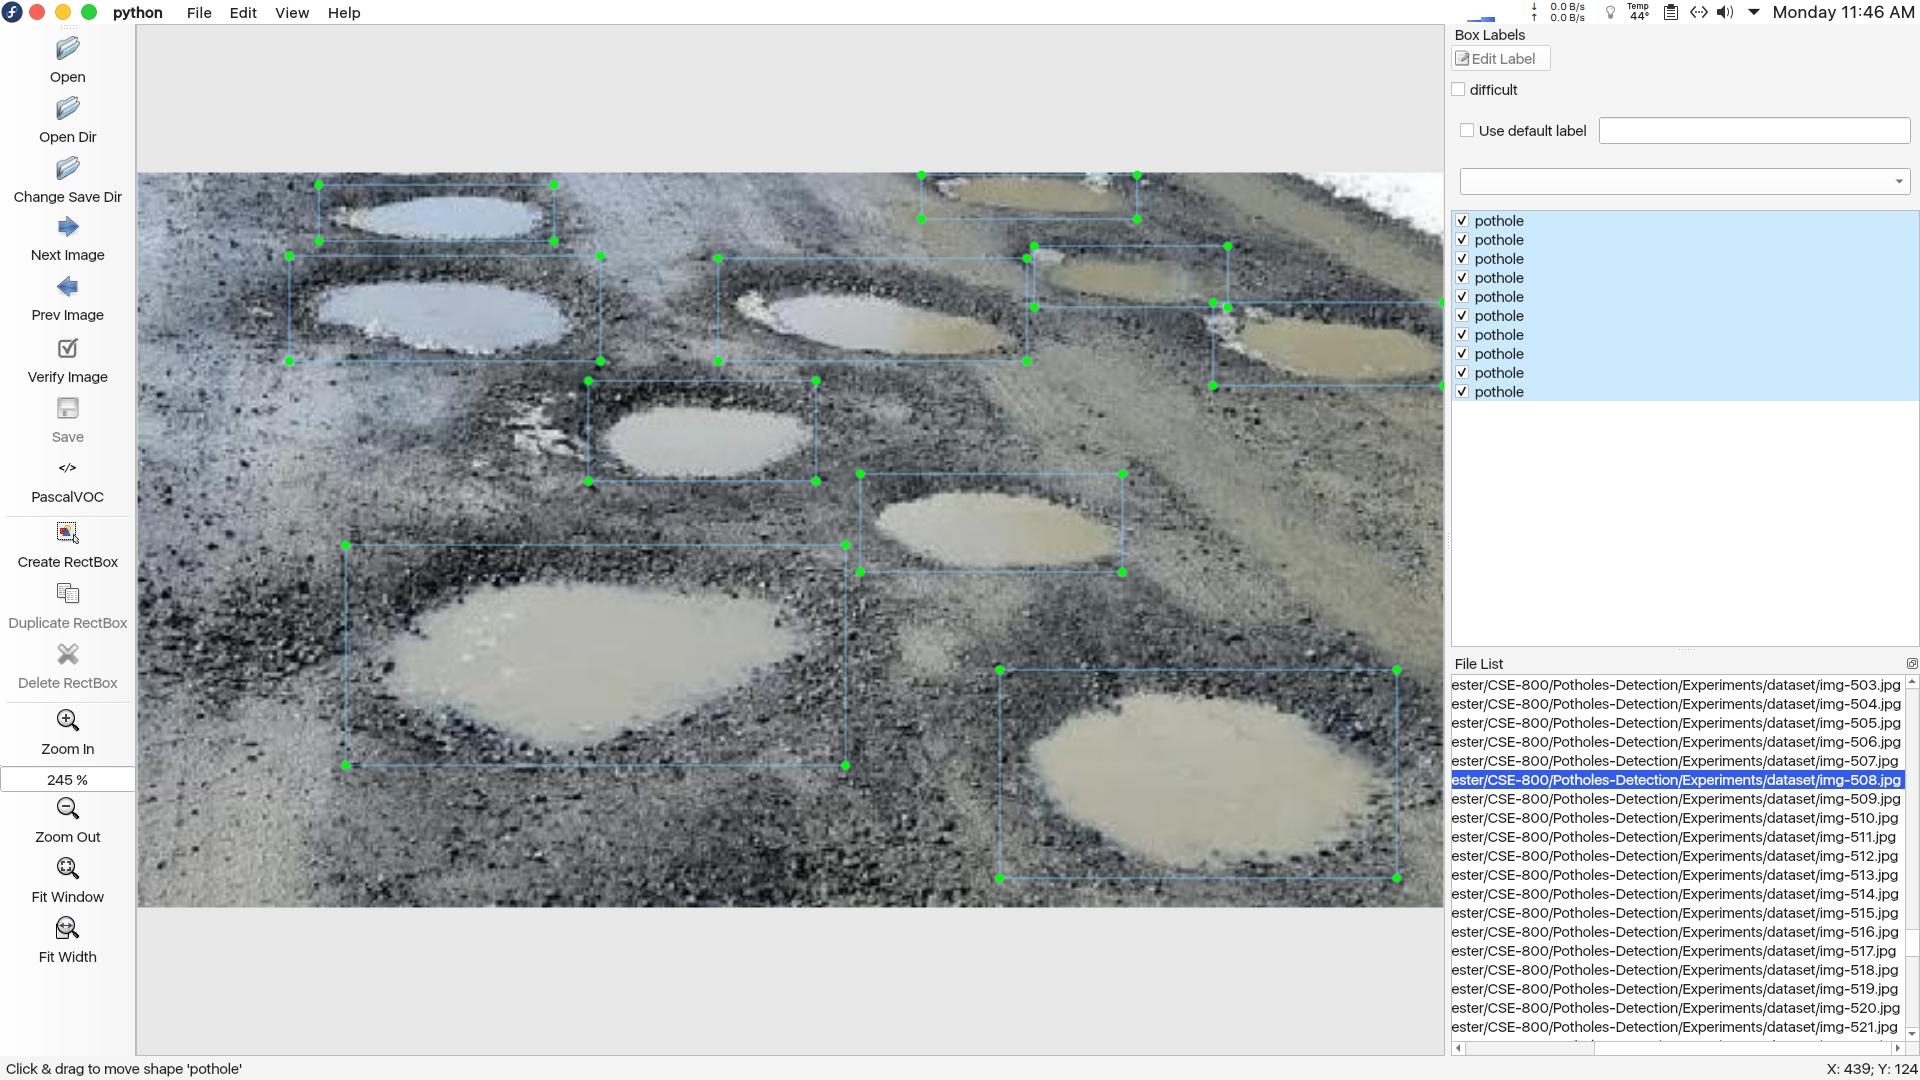
\includegraphics[width=\textwidth]{images/labelImg.png}
                \caption{Selecting the Regions of Interest using labelImg}
                \label{fig:labelImg}
            \end{figure}
            
        \subsection{Splitting the Dataset into Train an Validation}
            We have partitioned all the annotated images into two disjoint sets. The set of training data contains 80\% of the total dataset and the set of validation data contains the rest 20\% of total dataset.
            
            \begin{figure}
                \centering
                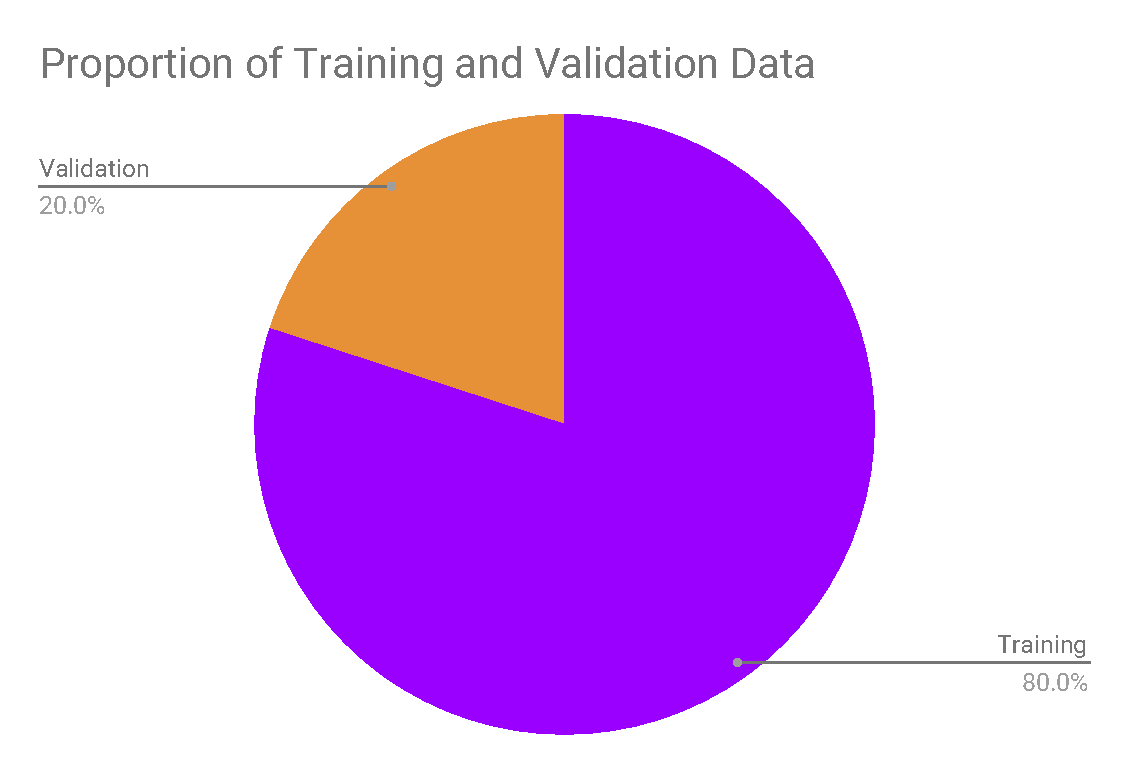
\includegraphics[width=\textwidth]{images/Proportion of Training and Validation Data.pdf}
                \caption{Proportion of Training and Validation Data}
                \label{fig:train_test_proportion}
            \end{figure}
        
            \begin{table}
                \centering
                \begin{tabular}{|c|c|c|} \hline
                     &  Number of Images & Percentage \\\hline\hline
                    Training & 532 & 80\% \\\hline
                    Validation & 113 & 20\% \\\hline
                \end{tabular}
                \caption{Proportion of Training and Validation Data}
                \label{tab:train_test_proportion}
            \end{table}
            
            This partitioning was followed by random splitting. The code we used to do this task is given in Appendix \ref{A.1}.
            
        \subsection{Creating tfrecord Files}
            Tensorflow Object Detection \acrshort{api} uses \gls{tfrecord} file format bundling all the dataset-images along with their regions of interest and class-labels. Therefore, we can feed the tfrecord generated from our dataset. We created two separate tfrecord files-- one for training dataset and another for validation dataset.
            
            Python Code to create \gls{tfrecord} files is given in Appendix \ref{A.2}.
            
    \section{Preparing a Pre-Trained Model}
        We have followed transfer learning approach in this research experiment. So, we required a pre-trained model ready to be used as a base model. There are many pre-trained models trained on different datasets with different metrics. These pre-trained models can be found in Tensorflow Model Zoo.
        
        We have used the \acrshort{ssd} MobileNet V2 pre-trained model which was trained on Microsoft \acrshort{coco} dataset.
        
        \subsection{Fine-Tune Configuration}
            Every pre-trained model in the Tensorflow Model Zoo contains a ``pipeline.config'' file which is used as a configuration file during training and evaluation. We have removed/changed/added several configuration options in that file. Our changes is shown in table.
            
            Example of some options the configuration file consists are---
            \begin{itemize}
                \item {Number of classes/labels}
                \item {Activation Functions}
                \item {Prepossessing Data Augmentation Options}
                \item {Learning Rate and Batch Size}
                \item {Evaluation Methods}
            \end{itemize}
